The environment used is a $47\times115$ grid-world with layout similar to the one used in \cite{wurman2008coordinating}. The agents are to collaboratively deliver $1183$ boxes to their designated delivery point, see implementation details [ref].

The numerical results are based on running cooperative
A* and multiagent rollout for 200 episodes for each agent
count, where an episode is determined complete when
all of the boxes are successfully delivered. Moreover, an
Apple M1 processor was used for all simulations and was
performed on a single thread.
\subsection{Runtime and memory consumption}

\definecolor{color1}{rgb}{0, 0.4470, 0.7410}
\definecolor{color2}{rgb}{0.8500, 0.3250, 0.0980}
\definecolor{color3}{rgb}{0.4660, 0.6740, 0.1880}
\tikzset{plotline/.style={line width=0.9}}
\tikzset{plotline1/.style={plotline, color=color1, mark=square}}
\tikzset{plotline2/.style={plotline, color=color2, mark=*}}
\tikzset{plotline3/.style={plotline, color=color3, mark=triangle}}

\begin{figure}
    \centering
    \vspace{1.6mm}
    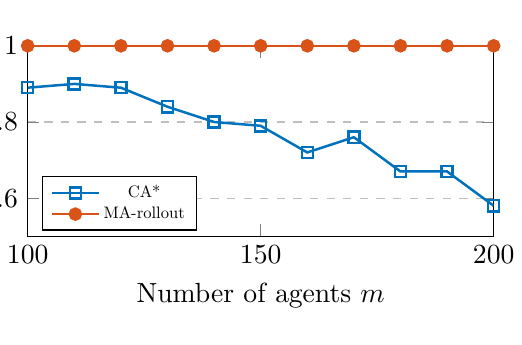
\begin{tikzpicture}[trim axis left, trim axis right]
    \begin{axis}[
        xlabel={Number of agents $m$},
        ylabel={Success rate},
        xmin=100, xmax=200,
        ymin=0.5, ymax=1,
        width=7.5cm,
        height=4cm,
        xtick={100,150,200},
        ytick={},
        legend pos=south west,
        ymajorgrids=true,
        grid style=dashed,
        legend style={nodes={scale=0.6, transform shape}},
    ]
    
    \addplot[
        plotline1,
        ]
        coordinates {
        (100, 0.89)(110,0.9)(120,0.89)(130,0.84)(140,0.80)(150,0.79)(160, 0.72)(170, 0.76)(180, 0.67)(190, 0.67)(200, 0.58)
        };
    \addlegendentry{CA*}
    
    \addplot[
        plotline2,
        ]
        coordinates {
        (100, 1)(110,1)(120,1)(130,1)(140,1)(150,1)(160, 1)(170, 1)(180, 1)(190, 1)(200, 1)
        };
    \addlegendentry{MA-rollout}
        
        
    \end{axis}
    \end{tikzpicture}
        \caption{The average rate at which the methods are able to produce a feasible path.}
        \vspace{2mm}
        \label{fig:success_rate}
\end{figure}

\begin{figure}
    \centering

    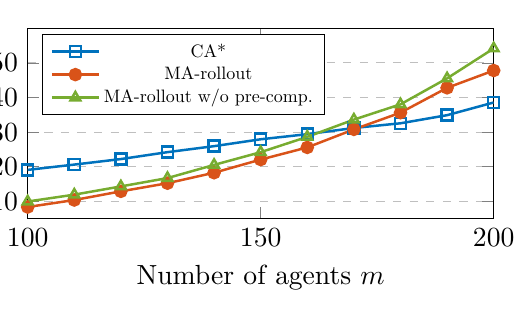
\begin{tikzpicture}[trim axis left, trim axis right]
    \begin{axis}[
        xlabel={Number of agents $m$},
        ylabel={Runtime [ms]},
        xmin=100, xmax=200,
        ymin=5, ymax=60,
        width=7.5cm,
        height=4cm,
        xtick={100,150,200},
        ytick={10, 20, 30, 40, 50},
        legend pos=north west,
        ymajorgrids=true,
        grid style=dashed,
        legend style={nodes={scale=0.65, transform shape}},
    ]
    
    \addplot[
        plotline1,
        ]
        coordinates {
        (100, 19.0847)(110,20.6146)(120,22.2105)(130,24.2083)(140,25.9375)(150,27.9247)(160, 29.4)(170, 31.1875)(180, 32.5426)(190, 34.8866)(200, 38.5506)
        };
    \addlegendentry{CA*}
        
    \addplot[
        plotline2,
        ]
        coordinates {
        (100, 8.35895)(110,10.3783)(120,12.8847)(130,15.2359)(140,18.2616)(150,22.0642)(160, 25.5706)(170, 30.7799)(180, 35.61)(190, 42.7839)(200, 47.7844)
        };
    \addlegendentry{MA-rollout}
    
    \addplot[
        plotline3,
        ]
        coordinates {
        (100, 9.95)(110,11.93)(120,14.31)(130,16.7216)(140,20.5228)(150,24.1993)(160, 28.6255)(170, 33.6049)(180, 38.0182)(190, 45.5216)(200, 54.16)
        };
    \addlegendentry{MA-rollout w/o pre-comp.}
        
        
    \end{axis}
    \end{tikzpicture}
        \caption{The average time it takes to obtain  controls for all agents.}
        \label{fig:runtime}
\end{figure}

\begin{figure}
    \centering

    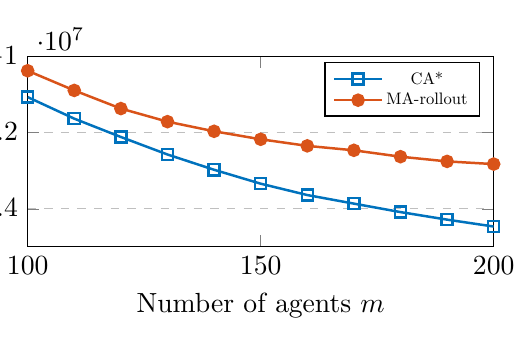
\begin{tikzpicture}[trim axis left, trim axis right]
    \begin{axis}[
        xlabel={Number of agents $m$},
        ylabel={$J_{\Tilde{\mu}}$},
        xmin=100, xmax=200,
        ymin=-15000000, ymax=-10000000,
        width=7.5cm,
        height=4cm,
        xtick={100,150,200},
        ytick={},
        legend pos=north east,
        ymajorgrids=true,
        grid style=dashed,
        legend style={nodes={scale=0.6, transform shape}},
    ]
    
    \addplot[
        plotline1,
        ]
        coordinates {
        (100, -11067000)(110,-11633200)(120,-12114500)(130,-12573800)(140,-12974900)(150,-13340400)(160, -13638800)(170, -13864100)(180, -14086000)(190, -14284500)(200, -14465500)
        };
    \addlegendentry{CA*}
    
    \addplot[
        plotline2,
        ]
        coordinates {
        (100, -10375300)(110,-10891900)(120,-11368100)(130,-11711800)(140,-11964700)(150,-12174700)(160, -12347200)(170, -12464300)(180, -12631600)(190, -12755200)(200, -12825800)
        };
    \addlegendentry{MA-rollout}
        
        
    \end{axis}
    \end{tikzpicture}
        \caption{The cumulative cost $J_{\Tilde{\mu}}$, averaged over 200 episodes. This is far smaller than $\Tilde{J}$, which has an average value of around $10^{20}$, verifying inequality \eqref{eq:cost_bound}.}
        \vspace{2mm}
        \label{fig:cumulative_reward}
\end{figure}

\begin{figure}
    \centering

    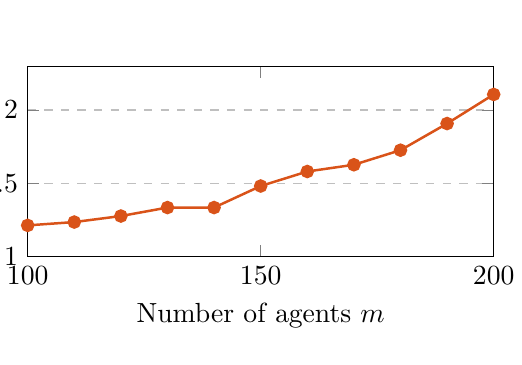
\begin{tikzpicture}[trim axis left, trim axis right]
    \begin{axis}[
        xlabel={Number of agents $m$},
        ylabel={Number of reshuffles},
        xmin=100, xmax=200,
        ymin=1, ymax=2.3,
        width=7.5cm,
        height=4cm,
        xtick={100,150,200},
        ytick={},
        legend pos=north east,
        ymajorgrids=true,
        grid style=dashed,
        legend style={nodes={scale=0.6, transform shape}},
    ]
    
    \addplot[
        plotline2,
        ]
        coordinates {
        (100, 1.2124)(110,1.23507)(120,1.27614)(130,1.3341)(140,1.3341)(150,1.48104)(160, 1.58021)(170, 1.62622)(180, 1.72564)(190, 1.90758)(200, 2.10627)
        };
        
        
    \end{axis}
    \end{tikzpicture}
        \caption{The average number of reshuffles needed. (MAYBE REMOVE?)}
        \vspace{2mm}
        \label{fig:number_of_shuffles}
\end{figure}


It is clear from Fig. \ref{fig:runtime} that Cooperative A* is slightly faster than multiagent rollout when there are more than 160 agents. However, one has to consider the lower success rate of Cooperative A* since only the successful computations runtime is part of the average. Furthermore, due to the parallel nature in which the approximations of the costs of each agent's controls are evaluated, one can imagine that it would be, in theory, possible to reduce the runtime of multiagent rollout by a factor of $C=5$ by doing these computations in parallel.


Additionally, the scale of the graph in which the shortest-path search is performed, differs between the methods. The graph needed by Cooperative A* is expected to be $N$ times larger than the graph used by the base policy of multiagent rollout, where $N$ denotes the time-steps needed for the agent to reach the target. This may therefore pose limitations on the maximum path-length of Cooperative A* from a memory standpoint.
\subsection{Adaptability}
Since the real-life operation of a warehouse is prone to unforeseen events, like robot malfunctioning, it is of great importance for a warehouse path-finding algorithm to be able to adapt to these circumstances. To investigate multiagent rollout's adaptability, we purposely simulated the total loss of control of some robots. More precisely, up to $20\%$ of robots were intentionally unable to move and the other agents regarded the grounded robots as having their base policy changed to one of complete stand-still. Remarkably, multiagent rollout adapted to this scenario, and the remaining agents continued their operation by circumnavigating these malfunctioned robots.